\documentclass{article}
%\usepackage[proof]{jmb}
\usepackage{jmb}
\usepackage{a4}
\usepackage{rotating}
\usepackage{epsfig}

\newcommand{\degrees}{\mbox{${}^{\circ}$}}
\newcommand{\htt}{\mbox{$3_{10}$}}
\newcommand{\tick}{\mbox{$\surd$}}
\newcommand{\Asq}{\mbox{\AA${}^{2}$}}

\emergencystretch 1in

\title{The ups and downs of protein topology; rapid comparison of protein
structure\\
{\large {\bfseries Running title:} The ups and downs of protein topology}\\
{\large {\bfseries Keywords:} structure comparison; protein fold;
CATH; structural similarity}}
\author{Andrew C.R.\ Martin\\
School of Animal and Microbial Sciences\\
University of Reading\\
Whiteknights\\
P.O.~Box~228, Reading RG6 6AJ, U.K.\\
Tel.: +44 (0)118 987 5123 Extn. 7022\\
Fax: +44 (0)118 931 0180 \\
EMail: a.c.r.martin@reading.ac.uk}

\begin{document}
\maketitle
\bibliographystyle{jmbacrm}

%%%%%%%%%%%%%%%%%%%%%%%%%%%%%%%%%%%%%%%%%%%%%%%%%%%%%%%%%%%%%%%%%%%%%%%%%
\begin{abstract}
Protein topology can be described at different levels. At the most
fundamental level, it is a sequence of secondary structure elements (a
``primary topology string''). Searching predicted primary topology
strings against a library of strings from known protein structures is
the basis of some protein fold recognition methods.  Here a method
known as TOPSCAN is presented for rapid comparison of protein
structures. Rather than a simple 2-letter alphabet (encoding strand
and helix), more complex alphabets are used encoding direction,
proximity, accessibility and length of secondary elements and loops in
addition to secondary structure.  Comparisons are made between the
structural information content of primary topology strings and
encodings which contain additional information (``secondary topology
strings'').  The algorithm is extremely fast, with a scan of a large
domain against a library of more than 2000 secondary structure strings
completing in around 30 seconds. Analysis of protein fold similarity
using TOPSCAN at primary and secondary topology levels is presented.
\end{abstract}

%%%%%%%%%%%%%%%%%%%%%%%%%%%%%%%%%%%%%%%%%%%%%%%%%%%%%%%%%%%%%%%%%%%%%%%%%
\section{Introduction}
As rapidly increasing quantities of new structure data become
available, the classification of protein folds is becoming more and
more important. When a new structure is solved, one wishes to ask the
question of whether this fold has been seen before. If the fold is one
of the commonly occurring superfolds (e.g.\ immunoglobulin-fold, TIM
barrel, $\alpha\beta$-plait, Rossmann fold), then it can generally be
recognised by eye, but the less common folds are more difficult to
recognise. Outside these superfolds, there is generally a one-to-one
mapping between fold and homologous family.  In some cases, remote
homologues may only be recognised in the light of structural
similarity allowing inference of functional information.  Automated
servers to answer the classification question have recently been
developed and rely on structure comparison programs.

Unfortunately, detailed automatic structure comparison is a
time-consuming process. The double-dynamic programming algorithm used
in SSAP\cite{taylor:alignment} at the atomic coordinate level is
particularly computer intensive making it impractical to run a full
scan of a protein of any size against a library of known folds.  An
experimental ``CATH-server'' at University College
London\cite{orengo:classifying} has made use of sequence screening and
a hierarchical expansion scheme through the representative levels in
the CATH domain classification database\cite{orengo:cath} to reduce
the search, but in the worst case scenario, it could still be
necessary to scan against more than 3000 near-identical sequence
representatives. It is estimated that approximately 2 weeks of computer time
would be required to scan a large protein domain such as a TIM barrel
in this way and this is clearly impractical for use as a server. The
initial goal of this work therefore was to develop a rapid approximate
method for protein fold comparison which could be used as a pre-screen
for SSAP.

The CATH classification of protein domain structures is a hierarchical
classification encoding class (C), architecture (A), topology (T),
homology (H), sequence family (S), near-identical sequence (N) and
identical sequence (I). The use of the word ``topology'' in this
description is something of a misnomer. When we refer to the topology
of a protein, what we generally mean is the three-dimensional
fold. More strictly, for a given spatial arrangement of secondary
structure elements (SSEs), the topology describes how these elements
are connected.

The dictionary definition of ``topology'' is the factors which remain
unchanged as an object undergoes a continuous deformation.  In terms
of protein secondary structure, the true topology is simply the
sequence of SSEs.  i.e.\ if one imagines being able to hold the N- and
C-terminal ends of a protein chain and pull it out straight, the
topology does not change whatever the protein fold (providing no knots
are formed in the folded protein).  Here, we describe this as the
``primary topology'' while, by analogy with primary and tertiary
structure, the protein fold is described as the ``tertiary
topology''. A primary topology string is a sequence of E and H
characters representing $\beta$-strand and $\alpha$-helix in DSSP
notation\cite{kabsch:dictionary}.

When a sequence for a protein of unknown structure does not show
obvious sequence homology with a protein of known structure, fold
recognition is commonly used to give clues as to the three-dimensional
structure. There are two common approaches to this problem: one is
``threading'' which assesses how well a sequence is accommodated
within a three-dimensional structure\cite[for
example]{jones:threading}; the other is alignment of a predicted
sequence of SSEs against a fold library encoded in this form\cite[for
example]{russell:foldrec,rost:foldrec}.  These fold recognition
methods are therefore making the assumption that the tertiary topology
can be predicted from the primary topology. An analysis of the
occurrence of given primary topologies in different tertiary
topologies is presented.

If this assumption is true, then it should also be possible to use
primary topology strings for three-dimensional structure comparison.
However, given the extra information available within a
three-dimensional structure, one can introduce an intermediate level
of topology ``secondary topology'' which contains additional
information (such as SSE direction, proximity, accessibility and
length of the elements and the loops which connect them) to improve
the mapping between these lower levels of topological description and
tertiary topology (i.e.\ protein fold).

TOPSCAN was initially developed as a simple method to reduce the
search space for the CATH-server. In that implementation, the secondary
topology strings contain only the directional information.  It is used
to sort domains and SSAP is then used to make the final selection
working down the TOPSCAN-sorted list. In this way, we can be sure that
we will not miss any hits which might otherwise have been found using
a full search with SSAP alone.

Here an analysis of protein fold similarity at the primary and
secondary topology levels is presented and the ability of these to
predict similarity at the tertiary topology level is assessed.
Implications of the results for fold recognition and secondary
structure prediction are discussed.

%%%%%%%%%%%%%%%%%%%%%%%%%%%%%%%%%%%%%%%%%%%%%%%%%%%%%%%%%%%%%%%%%%%%%%%%%
\section{Results and Discussion}
%\input results.tex
%\input best.tex
%\input worst.tex
%\input bars.tex

\subsection{Assignment of secondary structure (primary topology)}
The assignment of secondary structure is the critical first stage. We
have found that the DSSP algorithm\cite{kabsch:dictionary} can be
over-sensitive to errors in the structure. For example, NMR structures
often show little secondary structure in DSSP assignments whereas an
intuitive visual inspection shows substantial secondary structure. The
DSSP algorithm works by assigning a cutoff to hydrogen-bonding
energies and finding patterns of hydrogen bonds characteristic of
secondary structures. Any hydrogen-bonds which fail to meet these
criteria are excluded and secondary structure assignment may therefore
be less than optimal.

The STRIDE software from Argos and co-workers\cite{frishman:ssassign} was
designed to reduce this sensitivity. However, using STRIDE in place of
DSSP makes little difference to the overall results (data not
shown). The TOPSCAN software allows either DSSP or STRIDE secondary
structure assignments to be used and STRIDE was selected for all
further analysis.

% The simplified secondary structure assignment scheme used within
% RasMol actually appears to perform better in assigning secondary
% structures in an intuitive manner and we are investigating the
% possibility of extracting this code from RasMol for stand-alone
% secondary structure assignment.

We explored the effects of setting the minimum required number of
consecutive residues assigned to a given secondary structure to 3 and
4 residues. We also looked at treating \htt\ helix residues as the
same as $\alpha$-helix (data not shown). This made little difference
when the length cutoff was set to 4, but made results significantly
worse when the length cutoff was set to 3. This is because most
instances of true \htt\ helix are $<4$ residues in length (as shown
above, the mean length of a \htt-helix is 3.3 residues). These are
then treated as $\alpha$-helix and compared with regions of true
$\alpha$-helix.  The implication here is that treating \htt\ helix as
$\alpha$-helix is not a good strategy and this has implications for
those who do this in secondary structure prediction\cite[for
example]{king:combine}. It appears that it would be better to treat
\htt-helix as coil in secondary structure prediction, particularly
when this is being used for fold recognition.


%11111111111111111111111111111111111111111111111111111111111111111111111
\subsection{Assignment of secondary topology}
In addition to secondary structure and the direction of SSEs, 
following factors were considered in defining secondary topology:
accessibility, proximity, element length and loop length. The
performance is assessed in terms of percent coverage vs.\ percent
error, specifically taking error rates of 1\% and 5\%. These results
are summarised in \tableref{\ref{tab:summary}}.

\begin{table}
\caption{\label{tab:summary}Summary of effects of adding information
to the secondary topology strings.}
\begin{tabularx}{\linewidth}{lllllXX} \hline
SS length &               &           & Element & Loop   & \multicolumn{2}{c}{Coverage} \\ \cline{6-7}
cutoff    & Accessibility & Proximity & length  & length & 1\% error & 5\% error \\ \hline
3         &               &           &         &        & 16.55     & 47.14     \\
3         &               &           &         & \tick  & 17.89     & 48.02     \\
3         &               &           & \tick   &        & 20.85     & 49.35     \\
3         &               &           & \tick   & \tick  & 22.06     & 49.80     \\
3         &               & \tick     &         &        & 18.55     & 48.43     \\
3         &               & \tick     &         & \tick  & 19.97     & 48.71     \\
3         &               & \tick     & \tick   &        & 22.72     & 50.36     \\
3         &               & \tick     & \tick   & \tick  & 24.24     & 50.45     \\
3         & \tick         &           &         &        & 19.84     & 49.54     \\
3         & \tick         &           &         & \tick  & 21.14     & 49.92     \\
3         & \tick         &           & \tick   &        & 23.87     & 51.46     \\
3         & \tick         &           & \tick   & \tick  & 24.92     & 51.37     \\
3         & \tick         & \tick     &         &        & 21.74     & 50.32     \\
3         & \tick         & \tick     &         & \tick  & 23.17     & 50.23     \\
3         & \tick         & \tick     & \tick   &        & 25.59     & 51.92     \\
3         & \tick         & \tick     & \tick   & \tick  & 26.43     & 51.75     \\
          &               &           &         &        &           &           \\
4         &               &           &         &        & 15.67     & 45.07     \\
4         &               &           &         & \tick  & 17.12     & 45.48     \\
4         &               &           & \tick   &        & 20.26     & 47.01     \\
4         &               &           & \tick   & \tick  & 20.95     & 47.39     \\
4         &               & \tick     &         &        & 17.74     & 46.26     \\
4         &               & \tick     &         & \tick  & 19.27     & 46.53     \\
4         &               & \tick     & \tick   &        & 22.11     & 47.79     \\
4         &               & \tick     & \tick   & \tick  & 22.87     & 47.70     \\
4         & \tick         &           &         &        & 19.17     & 47.41     \\
4         & \tick         &           &         & \tick  & 20.25     & 47.44     \\
4         & \tick         &           & \tick   &        & 22.72     & 48.59     \\
4         & \tick         &           & \tick   & \tick  & 23.46     & 48.69     \\
4         & \tick         & \tick     &         &        & 20.86     & 48.22     \\
4         & \tick         & \tick     &         & \tick  & 22.11     & 47.75     \\
4         & \tick         & \tick     & \tick   &        & 24.39     & 49.01     \\
4         & \tick         & \tick     & \tick   & \tick  & 25.02     & 48.98     \\
\hline
\end{tabularx}
Coverage values at 1\% and 5\%
error rates were calculated by linear interpolation of the coverage
vs. error plots in the ranges 0.5--1.75 and 3.0--8.0
respectively. This gives a sample of approximately 8 points evenly
spread above and below the interpolation point.
\hrule
\end{table}

As seen in the table, the best coverage results are achieved with the
secondary structure cutoff set to 3 and with accessibility, proximity,
element length and loop length information in the secondary topology
strings.  Interestingly, at the 5\% error rate, loop length has a
detrimental effect, presumably because the loops are the most variable
factor between proteins adopting the same fold.


%11111111111111111111111111111111111111111111111111111111111111111111111
% -----------------------------------------------------
%                  Primary                Secondary
%               ---------------         ---------------
%               Within  Between         Within  Between
% -----------------------------------------------------
% ...All...
% >95           51      30723           9       812
% >65           258     667151          107     6839           
% >60           269     970672          125     12282
% >55           276     1312787         169     27754
% >50           281     1655551         205     62808
% Observations: 292     4688807         292     4688807
%
% ...>3 SSEs...
% >95           41      28944           3       64
% >65           238     665372          93      5112
% >60           247     968893          111     10555
% >55           252     1311008         151     26027
% >50           255     1653772         185     61081
% Observations: 259     4495340         259     4495340
% -----------------------------------------------------

\begin{table}
\caption{\label{tab:scores} High scoring comparisons.}
\begin{center}
\begin{tabularx}{\linewidth}{Xlllll}\hline
              & \multicolumn{2}{c}{Primary} & & \multicolumn{2}{c}{Secondary} \\ \cline{2-3}\cline{5-6}
Score (\%)    & Within    & Between         & & Within    & Between           \\ \hline
\multicolumn{6}{l}{\bfseries All structures} \\
$>95$         & 17.5\%    & 0.66\%          & & 3.08\%    & 0.02\%            \\
$>65$         & 88.4\%    & 14.2\%          & & 36.6\%    & 0.15\%            \\ 
$>60$         & 92.1\%    & 20.7\%          & & 42.8\%    & 0.33\%            \\ 
$>55$         & 94.5\%    & 28.0\%          & & 57.9\%    & 0.59\%            \\ 
$>50$         & 96.2\%    & 35.3\%          & & 70.2\%    & 1.34\%            \\ 
Observations: & 292       & 4688807         & & 292       & 4688807           \\
              &           &                 & &           &                   \\
\multicolumn{6}{l}{\bfseries $>3$ secondary structure elements} \\
$>95$         & 15.8\%    & 0.64\%          & & 1.16\%    & 0.001\%           \\
$>65$         & 91.9\%    & 14.8\%          & & 35.9\%    & 0.11\%            \\ 
$>60$         & 95.4\%    & 21.6\%          & & 42.9\%    & 0.23\%            \\ 
$>55$         & 97.3\%    & 29.2\%          & & 58.3\%    & 0.58\%            \\ 
$>50$         & 98.4\%    & 36.8\%          & & 71.4\%    & 1.36\%            \\ 
Observations: & 259       & 4495340         & & 259       & 4495340           \\ \hline
\end{tabularx}
\end{center}
Percentage of comparisons scoring above cutoffs of 50\%, 55\%, 60\%,
65\% and 95\% first for comparisons of all structures and second only
for comparisons of topology strings containing 4 or more secondary
structure elements (SSEs).  \hrule
\end{table}

\subsection{Does primary topology predict protein fold?}
Using the CATH classification, each protein fold containing more than
one near-identical sequence family (i.e.\ each CAT level containing
more than one Nrep) was examined. Within each of these 292 groups, the
mean TOPSCAN score was calculated for all pairs of Nreps using only
the primary topology (secondary structure cutoff length set to 3).
The frequency of scores obtained is shown in
\figref{\ref{fig:primary}a}.  Unsurprisingly, the highest peak is for
a score of 95--100\% (see \tableref{\ref{tab:scores}}), i.e.\ within a
protein fold, the primary topology is generally identical. As shown in
the table, similar results were obtained when trivial matches between
very small structures containing fewer than 4 SSEs were ignored.

\begin{figure}
\begin{tabular}{ll}
a                               & b                             \\
\epsfig{file=pics/within_primary.mean.ps,width=2.5in} & %
\epsfig{file=pics/between_primary.ps,width=2.5in} \\
\end{tabular}
\caption{\label{fig:primary}Frequency of scores achieved using primary
topology a) within a given protein fold b) when comparing a given fold
with every other fold.}
\end{figure}

\begin{figure}
\begin{tabular}{ll}
a                               & b                             \\
\epsfig{file=pics/1aca.ps,width=2.5in} & \epsfig{file=pics/2ccy.ps,width=2.5in} \\
\end{tabular}
%\centerline{\epsfig{file=pics/1aca.ps,width=3in}\epsfig{file=pics/2ccy.ps,width=3in}}
\caption{\label{fig:4helix}Two examples of 4-helix bundles: a) PDB
code: 1aca and b) PDB code: 2ccy chain A.  Both would have the same
primary topology description of HHHH, but they show different
topologies (CATH topology assignments 1.20.80 and 1.20.120
respectively). The four helices are coloured blue, green, orange, red
working from N-terminus to C-terminus. Images were generated with 
Molscript~2.1.2\protect\cite{kraulis:molscript}}
\end{figure}

Every Nrep within each protein fold (CAT) was then compared with every
Nrep of every other protein fold (a total of 4688807 comparisons) and
the distribution of the scores was plotted
(Figure~\ref{fig:primary}b).  Initially one would expect that
different folds will have a low score in this comparison, but 14.2\% of
the comparisons score $>65\%$ with 0.66\% scoring $>95\%$ (see
Table~\ref{tab:scores}), the distribution peaking at a score of
35--40\%.  However when one considers, for example, 4-helix bundles as
shown in \figref{\ref{fig:4helix}}, it becomes obvious that there are
multiple folds containing the same set of SSEs. The figure shows two
4-helix bundles from bovine acyl-coenzyme~A binding protein\cite[PDB
code: 1aca]{kragelund:1aca} and cytochrome~C$'$ from
\emph{Rhodospirillum molischianum}\cite[PDB code:
2ccy]{finzel:2ccy}. At the primary topology level, both would be
described as HHHH (note that 2ccy has a short segment of \htt\ helix
between the second and third main helices).

Thus, by knowing only the primary topology (perhaps from
secondary structure prediction), there is a high chance of matching
the incorrect protein fold with an identical primary topology.

\begin{figure}
\begin{tabular}{ll}
a                               & b                             \\
\epsfig{file=pics/within_secondary.mean.ps,width=2.5in} & %
\epsfig{file=pics/between_secondary.ps,width=2.5in} \\
\end{tabular}
\caption{\label{fig:secondary}Frequency of scores achieved using
secondary topology a) within a given protein fold b) when comparing a
given fold with every other fold.}
\end{figure}

%11111111111111111111111111111111111111111111111111111111111111111111111
\subsection{Does secondary topology predict protein fold?}
As with comparison of primary topology, each protein fold containing
more than one near-identical sequence family was examined. Within each
of these groups, the TOPSCAN score was calculated using the secondary
topology with a secondary structure length cutoff of 3 and including
accessibility, proximity, element length and loop length information
(\figref{\ref{fig:secondary}a}, Table~\ref{tab:scores}). The
distribution moves to the left compared with using primary topology
and the peak for 95--100\% is lost. This is largely a result of the
single cutoffs used to define seondary topology. Scores are
artificially reduced where two examples lie close to, but on either
side of, the cutoff. The distribution peaks ar around 55--60\%.

Comparison between protein folds (Figure~\ref{fig:secondary}b) now
peaks at a score of 15--20\% and all the high scoring peaks
are removed. Only 0.15\% of comparisons score $>65\%$ (Table~\ref{tab:scores}).

Referring again to Figure~\ref{fig:4helix}, although the primary
topology for the two folds is the same (HHHH), by following the chain
trace, it is clear that the directions of the helices is different
(1aca: up, down, down, up; 2ccy: up, down, up, down) and incorporating
this information into the secondary topology strings will distinguish
between the two folds.

\begin{figure}
\begin{tabular}{ll}
a                               & b                             \\
\epsfig{file=pics/1dar.ps,width=2.5in} & %
\epsfig{file=pics/1elo.ps,width=2.5in} \\
\end{tabular}
\caption{\label{fig:1dar1elo}Domain three of elongation factor G (EF-G)
from \emph{Thermus thermophilus} strain HB8 a) from crystal structure
1dar in complex with GDP and b) from crystal structure 1elo of the
free protein. The structures are coloured from blue at the N-terminus
(residue 433) to red at the C-terminus (residue 483). Note the
dicontinuities resulting from some residues not being visible
in the x-ray structures.}
\end{figure}

Interestingly both the comparisons of primary and secondary topology
within a fold show one comparison with a very low score ($<10$\%).
These structures (domain 3 from PDB files 1dar\cite{al-karadaghi:1dar}
and 1elo\cite{aevarsson:1elo}) were examined using RasMol and are
shown in \figref{\ref{fig:1dar1elo}}. They represent one domain from
elongation factor G (EF-G) from \emph{Thermus thermophilus} strain HB8
complexed and uncomplexed with GDP respectively. Whereas 1dar contains
only $\beta$-strands, 1elo has two poorly defined strands and a
helix. The sequences of these two are identical, yet the fold is
different as a result of conformational flexibility of EF-G on binding
nucleotide.  It should also be noted that the structures are poorly
defined in this region with some residues not visible in the crystal
structures. Thus some of the differences may reflect errors in the
structures although, since both structures are solved by the same
group, it is unlikely that they would have built one with an
$\alpha$-helix and the other without unless there were a real
difference.


%11111111111111111111111111111111111111111111111111111111111111111111111
\subsection{Problems}
The algorithm has problems in discriminating, for example, a TIM
barrel from a Rossmann fold. These are topologically somewhat similar
--- in both cases, they consist in the main of alternating
$\beta$-strands and $\alpha$-helices which form a core of
$\beta$-sheet with helices on the outside. In the case of the TIM
barrel the $\beta$-sheet is curved into a barrel whereas the Rossmann
fold has a relatively flat sheet. Because the differences between the
two occur in a plane perpendicular to the direction of the SSEs, the
current method does not distinguish reliably between these
architectures.

\tableref{\ref{tab:timros}} shows three examples of TIM barrels and
Rossman folds having almost identical primary topology. ALthough in
these cases the sceondary topology similarites are much lower, it can
be seen that the scores are relatively high for such different protein
folds.



\begin{table}
\caption{\label{tab:timros} Examples of TIM barrels and Rossman folds
with similar primary and secondary topology}
\begin{center}
\begin{tabularx}{\linewidth}{llXll}\hline
Fold$^{\dag}$ %
     & Domain     & Primary                   & Primary         & Tertiary        \\
     & identifier & topology                  & similarity (\%) & similarity (\%) \\ \hline
TIM  & 1ads00     & {\tt EEHEHEHEHEHEHEHHHH}  &                 &                 \\
ROS  & 1yveI1     & {\tt EEHEHEHEHEHEHEHEH-}  & 90.6            & 46.1            \\
     &            &                           &                 &                 \\
TIM  & 1tml00     & {\tt -HHEHEHEHHEHEHEEH}   &                 &                 \\
ROS  & 1vid00     & {\tt HHHEHEHEHHEHEHEE-}   & 93.8            & 51.9            \\
     &            &                           &                 &                 \\
TIM  & 1pii02     & {\tt HEHEHEHEEEHEEH}      &                 &                 \\
ROS  & 2reb01     & {\tt HEHEHEHEHEHEEE}      & 90.0            & 45.7            \\ \hline
\end{tabularx}
\end{center}
The PDB codes are:
1ads\protect\cite{wilson:1ads}, 
1yve\protect\cite{biou:1yve},
1tml\protect\cite{spezio:1tml},
1vid\protect\cite{vidgren:1vid},
1pii\protect\cite{wilmanns:1pii},
2reb\protect\cite{story:2reb}
$^{\dag}$TIM: TIM barrels (CATH code 3.20.20); ROS: Rossmann folds (CATH code 3.40.40).
\hrule
\end{table}



%% %% %% %% %% %% %% %% %% %% %% %% %% %% %% %% %% %% %% %% %% %% %% %% 
%% Give examples of topology strings for TIM and Rossmann            %%
%% %% %% %% %% %% %% %% %% %% %% %% %% %% %% %% %% %% %% %% %% %% %% %% 

%11111111111111111111111111111111111111111111111111111111111111111111111
\subsection{Comparison of TOPSCAN with other rapid methods}

Three methods similar in principle to TOPSCAN are
FAST-SSAP\cite{taylor:alignment}, a constraint programming (CP) method
based on TOPS diagrams\cite{David_Gilbert_David_Westhead} and TOP, a
least-squares fitting method\cite{lu:top}.

FAST-SSAP uses double dynamic programming to align vectors
representing the SSEs to compare two structures. The CP method uses a
4-letter alphabet to represent the two types of secondary structure
going either up or down and adds information about chirality and
hydrogen bonds between SSEs.  Comparison is performed by finding a
maximum common template and scoring the two structures against that
template.  TOP represents each SSE by its two end-points and then
performs iterative least squares fitting of this small number of
points to find an optimal match.

The simple approach taken by TOPSCAN allows a very significant speed
advantage. It is approximately 25$\times$ faster than the current
implementations of FAST-SSAP and CP and is estimated to be
approximately 30000$\times$ faster than normal SSAP.  FAST-SSAP could
be speeded by calculating the secondary structure vectors simply from
the end-points of the SSEs rather than using an Eigenvector.

Compared with FAST-SSAP, the simple segregation of secondary structure
vectors into six quadrants throws away a lot of more detailed
information about the relative orientation of the elements, but as a
result, allows us to perform normal single dynamic programming
removing the need for double dynamic programming.

Compared with CP, the TOPSCAN representation actually has more
information about directionality of the secondary structure vectors,
but loses the more detailed proximity information (encoded in the
constraint programming by hydrogen-bond information) and the chirality
arcs.

The authors of TOP do not provide directly comparable results.
However, since the method relies not only on the direction of the
SSEs, but also on the precise location of the endpoints, it seems
likely that the method will be particularly sensitive to the secondary
structure definition. It is well known that assignment is particularly
problematic at the ends of the secondary structures.

The best results achieved with TOPSCAN (c.26.5\% coverage at 1\% error
and c.52\% coverage at 5\% error) compare with c.60\% (at 1\% error)
and c.78\% (at 5\% error) for full SSAP and c.36\% (at 1\% error) and
c.58\% (at 5\% error) for CP\cite{gilbert:aisb}. Given the large
increase in speed achieved over these methods, TOPSCAN performs well
and is particularly valuable as a preliminary screen.

%%%%%%%%%%%%%%%%%%%%%%%%%%%%%%%%%%%%%%%%%%%%%%%%%%%%%%%%%%%%%%%%%%%%%%
\section{Conclusions}
TOPSCAN has proved a useful addition to the available methods for
comparing protein structures. In particular, it is useful as a
preliminary screen to look for possible similar structures. It also
provides a useful rapid method of ranking structures for further more
detailed comparison using SSAP.

Analysis of the CATH data has shown some interesting anomolies as well
as a few minor errors in the CATH data which have been fed back to the
CATH maintainers. Thus TOPSCAN also appears to have a role in rapid
validation of structural classification.

In common with the fast version of SSAP which relies on secondary
structure vectors and with CP and TOP which also make use of sequences
of SSEs, TOPSCAN is most likely to fail when a structure is poorly
defined and DSSP or STRIDE are unable to make reliable secondary
structure assignments. The atomic level full SSAP is less prone to
these problems, but pays a huge penalty in the time required for
comparison.

Future work will include investigating more complex classification of
properties such as solvent accessibility. Currently only binary
classifications are used (e.g.\ exposed vs. burried). In the case of
$\beta$-strands, specific allowance could be made for edge
strands. Changing the global Needlemann \& Wunsch dynamic programming
algorithm to a local Smith-Waterman alignment will also allow for
sub-structure matching. Given the current analysis of factors which
affect the accuracy of comparison of structures, this information can
feed back into fold recognition and the algorthim described here, when
combined with methods for prediction of the factors used in the
secondary topology string, will be of application in fold recognition.

%%%%%%%%%%%%%%%%%%%%%%%%%%%%%%%%%%%%%%%%%%%%%%%%%%%%%%%%%%%%%%%%%%%%%%%%%
\section{Materials and Methods}
TOPSCAN reduces a protein to a topology string which can represent the
structure as a string of letters encoding simply the primary topology
(a 2-letter alphabet) or the secondary topology using various
additional data from the 3D structure. For example, by encoding
direction information with the secondary structure, a 12-letter
alphabet is used.

A simple Needleman and Wunsch dynamic programming
algorithm\cite{needleman:wunsch} is then applied to compare two such
strings and a percentage similarity score is calculated.  The
percentage similarity score is calculated as the percentage of the
higher score achieved by scoring each of the two sequences against
itself.  Alternatively, rather than comparing two structures, a
library of topology strings may be pre-built from the Protein Databank
(or a representative subset) and a structure may then be scanned
against this library.

The TOPSCAN program itself is implemented in C. All analysis and
control of the programs was achieved using sets of scripts written in
Perl and driven from a relational database of the CATH data
implemented using the freely available object-relational database,
PostgreSQL (http://www.postgresql.org). Analysis was performed on a
dual PentiumIII-450 machine running RedHat Linux~6.0.

%11111111111111111111111111111111111111111111111111111111111111111111111
\subsection{Datasets}
All analysis was performed using datasets derived from the CATH
classification of protein domain folds\cite{orengo:cath}. In CATH,
representative structures are assigned at T, H, S and N levels.  For
analysis of parameters to be used in the program, the representatives
from the H level (Hreps) from CATH v1.6 were selected, but from this
set, any structures now obsoleted from the protein
databank\cite{berman:pdb} and any NMR structures were removed. This
gave a set of 914 domains representing a set of non-homologous protein
domains.

For testing the performance of the program, a similar set was created
using the CATH Nreps leading to a set of 3124 domains. Each Nrep is a
representative of a near identical group of sequences having $\ge
95$\% sequence identity. These were used to build the libraries
against which each of those 3124 domains was tested (matches against
self were always ignored in calculating results).


%11111111111111111111111111111111111111111111111111111111111111111111111
\subsection{Creating primary topology strings}
TOPSCAN enables secondary structure to be calculated from a
three-dimensional structure using either DSSP\cite{kabsch:dictionary}
or STRIDE\cite{frishman:ssassign}. For the analyses presented in this
paper, STRIDE was used.  From these assignments, regions of
$\beta$-sheet (Kabsch and Sander assignment, E) and of $\alpha$-helix
(Kabsch and Sander assignment, H) are extracted. Only continuous
regions of at least a specified number of residues with the same
assignment are selected.  This produces the primary topology of the
protein equivalent to a string of E and H characters where one
character represents one complete strand or helix. The program also
allows one to treat \htt\ helix assignments as $\alpha$-helix as is
frequently done in secondary structure prediction.

%11111111111111111111111111111111111111111111111111111111111111111111111
\subsection{Creating secondary topology strings}
To increase the information content of the topology string, various
information from the three-dimensional structure can be incorporated
into a secondary topology string. 

For simplicity and clarity of explanations, topology strings are
described here as vectors of characters. In practice, integer vectors
are used to allow more than 52 descriptors. This also provides a
technical simplification as lookups in the scoring matrix may be made
simply by the integer offsets for the two descriptors being compared.

%22222222222222222222222222222222222222222222222222222222222222222222222
\subsubsection{Secondary structure element (SSE) direction}
The end-points of each SSE in the primary topology are found in three
dimensions and the vector between them is calculated. The direction of
the vector is grouped into one of 6 classes depending on the largest
component of the vector (i.e.\ positive or negative $x$, $y$, or
$z$). This is equivalent to saying the element points up, down, left,
right, forward, or back. The encoding is summarised in
\tableref{\ref{tab:encoding}}.

\begin{table}
\caption{\label{tab:encoding}Encoding scheme used to represent
          secondary structure and direction information}
\begin{center}
\begin{tabularx}{\linewidth}{XXll} \hline
\multicolumn{2}{c}{Direction} & \multicolumn{2}{c}{Secondary Structure}\\ \cline{3-4}
          &         & strand & helix  \\ \hline
$+y$      & Up      & A      & G      \\
$+x$      & Right   & B      & H      \\
$-y$      & Down    & C      & I      \\
$-x$      & Left    & D      & J      \\
$+z$      & Back    & E      & K      \\
$-z$      & Forward & F      & L      \\ \hline
\end{tabularx}
\end{center}
\end{table}

The scoring matrix used for the dynamic programming algorithm is based
on the scoring scheme shown in \tableref{\ref{tab:matrix}}. While somewhat
arbitrary, it appears to work well: the same secondary structure in
the same orientation scores highest, different orientations score
worse and different secondary structure types achieve much lower
scores.

The starting premise was that for the same type of secondary
structure, one wishes to assign 3 scores: approximately the same
direction ($0\degrees\le\Delta\le 45\degrees$) scores 10,
approximately at right angles ($45\degrees\le\Delta\le 135\degrees$)
scores 5, approximately opposite ($135\degrees\le\Delta\le
180\degrees$) scores 2.  However, because of the boolean definition of
whether a vector is in a given quadrant, it is possible that vectors
actually point in very similar directions although they are in
different quadrants (for example one points at $+$44\degrees\ while
another points at $+$46\degrees; because the definition of quadrant
depends on the largest component of the direction vector, the quadrant
boundaries are at $\pm$45\degrees and $\pm$135\degrees). Picking pairs
of random numbers between 0--90 and 90--180 and plotting the
distribution of the differences shows an upside down V shaped curve
centred around 90 (data not shown). Two vectors in adjacent quadrants
will actually be within 90\degrees\ of one another 50\% of the
time. The actual score used for adjacent quadrants is therefore the
median of 10 and 5 ($7.5$ rounded up to 8).

%\begin{figure}
%\centerline{\epsfig{file=dist90.ps}}
%\caption{\label{fig:dist}Distribution obtained by picking 100000 pairs
%of numbers between 0--90 and 90--180 and plotting the differences.}
%\end{figure}

When two vectors are assigned to opposite quadrants, they can never be
closer than 90\degrees. Picking pairs of random numbers between 0--90
and 180--270 gives an identical distribution centred around 180. The
angle between two vectors can never be greater than 180\degrees, so
every angle $<$180\degrees\ observed between vectors in opposite
quadrants can also be seen in vectors assigned to adjacent quadrants.
In opposite quadrants, the angle between two vectors is
$<$135\degrees\ (our cutoff for saying two vectors are approximately
at right angles) $12.5$\% of the time. The score is therefore assigned
as $2+((5-2)\times 12.5/100) = 2\frac{3}{8}$ which is rounded back down
to 2.

For different secondary structure types, we make the simple arbitrary
assignments of 3, 1 and 0. A gap insertion penalty of 8 is used with
no gap extension penalty.

%% %% %% %% %% %% %% %% %% %% %% %% %% %% %% %% %% %% %% %% %% %% %% %% 
%% This really should be 3,2,0 - simply by applying the rule to the  %%
%% previous scores of ((3/8) * (x-2)) : such that we scale them to   %%
%% have 3 as a maximum score and 0 as a minimum.                     %%
%% %% %% %% %% %% %% %% %% %% %% %% %% %% %% %% %% %% %% %% %% %% %% %% 

% \begin{table}
% \begin{center}
% \begin{tabular}{rrrrrrrrrrrrr}
%   & A & B & C & D & E & F & G & H & I & J & K & L \\
% A &10 & 8 & 2 & 8 & 8 & 8 & 3 & 1 & 0 & 1 & 1 & 1 \\
% B & 8 &10 & 8 & 2 & 8 & 8 & 1 & 3 & 1 & 0 & 1 & 1 \\
% C & 2 & 8 &10 & 8 & 8 & 8 & 0 & 1 & 3 & 1 & 1 & 1 \\
% D & 8 & 2 & 8 &10 & 8 & 8 & 1 & 0 & 1 & 3 & 1 & 1 \\
% E & 8 & 8 & 8 & 8 &10 & 2 & 1 & 1 & 1 & 1 & 3 & 0 \\
% F & 8 & 8 & 8 & 8 & 2 &10 & 1 & 1 & 1 & 1 & 0 & 3 \\
% G & 3 & 1 & 0 & 1 & 1 & 1 &10 & 8 & 2 & 8 & 8 & 8 \\
% H & 1 & 3 & 1 & 0 & 1 & 1 & 8 &10 & 8 & 2 & 8 & 8 \\
% I & 0 & 1 & 3 & 1 & 1 & 1 & 2 & 8 &10 & 8 & 8 & 8 \\
% J & 1 & 0 & 1 & 3 & 1 & 1 & 8 & 2 & 8 &10 & 8 & 8 \\
% K & 1 & 1 & 1 & 1 & 3 & 0 & 8 & 8 & 8 & 8 &10 & 2 \\
% L & 1 & 1 & 1 & 1 & 0 & 3 & 8 & 8 & 8 & 8 & 2 &10 \\
% \end{tabular}
% \end{center}
% \caption{\label{tab:fullmatrix} Full scoring matrix for the 12-letter
% alphabet encoding protein topology.}
% \end{table}

\begin{table}
\caption{\label{tab:matrix} Scoring scheme employed in the matrix for
the dynamic programming comparison of two topology strings.}
\begin{center}
\begin{tabularx}{\linewidth}{Xll}\hline
                        & \multicolumn{2}{c}{Secondary structure} \\ \cline{2-3}
Orientation             & Same  & Different     \\ \hline
Same                    & 10    & 3             \\
Off by 1 quadrant       & 8     & 1             \\
Off by 2 quadrants      & 2     & 0             \\ \hline
\end{tabularx}
\end{center}
\end{table}



Because any pair of proteins is in an arbitrary relative orientation,
the definition of ``up'' in one protein may not correspond to ``up''
in the second. Therefore, one of the strings is permuted 23 times,
such that the dynamic programming algorithm comparison is performed a
total of 24 times (equivalent to the 6 sides of a cube, each of which
may be 4 ways up). \tableref{\ref{tab:permute}} shows the modifications
made to the encoding to achieve rotations about $x$, $y$ and $z$ axes.

\begin{table}
\caption{\label{tab:permute} Permutations to topology strings.}
\begin{center}
\begin{tabularx}{\linewidth}{XXXX}\hline
        & \multicolumn{3}{c} {Rotation axis} \\ \cline{2-4}
        & \multicolumn{1}{c}{$x$} %
                        & \multicolumn{1}{c}{$y$} %
                                        & \multicolumn{1}{c}{$z$} %
                                                        \\ \hline
Old     & ABCDEFGHIJKL  & ABCDEFGHIJKL  & ABCDEFGHIJKL  \\
New     & EBFDCAKHLJIG  & AECFDBGKILJH  & BCDAEFHIJGKL  \\ \hline
\end{tabularx}
\end{center}
To achieve a rotation about $x$, $y$ and $z$ axes, each
letter in the `Old' line is replaced by the letter immediately below
it in the `New' line.
\hrule
\end{table}




%22222222222222222222222222222222222222222222222222222222222222222222222
\subsubsection{Secondary Structure Element (SSE) Proximity}
To add information about the packing of SSEs, the proximity of an SSE
to the preceding element is encoded. This is performed as follows (see
\figref{\ref{fig:proximal}}).

\begin{figure}
\centerline{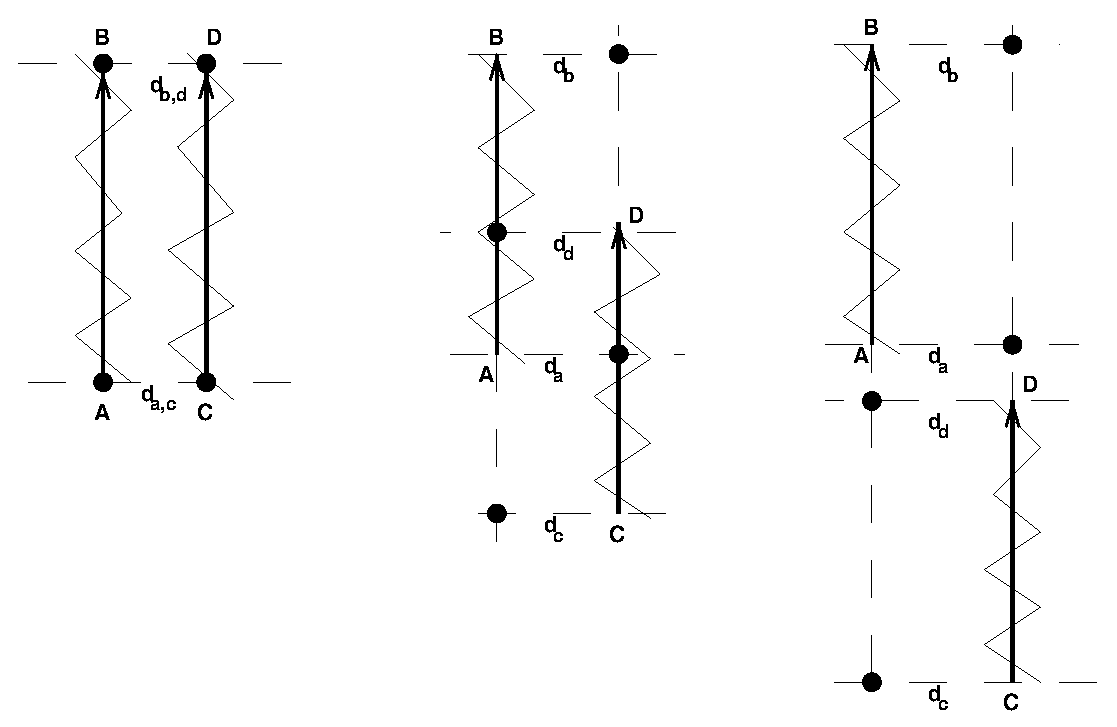
\psfig{file=neighbour.eps,width=\linewidth}}
\caption{\label{fig:proximal}Calculation of proximity of an SSE to the
preceding element. a) is considered proximal if $d_a$, $d_b$, $d_c$,
or $d_d$ is $<12.0$\AA; b) is considered proximal if $d_a$ or $d_d$ is
$<12.0$\AA; c) is not considered proximal because the nearest points
to $A,B,C$ and $D$ (shown by black circles) are not between the
secondary structure end points.}
\end{figure}

Given an element with endpoints C,D and a preceding element with
endpoints A,B, the minimum distances between points A and B and the
line described by CD are calculated.  This is repeated with points C
and D to line AB. As each minimum point-to-line distance is
calculated, the position on the line closest to the point is
calculated (shown in Figure~\ref{fig:proximal} with a black
circle). If this point is between the two endpoints of the line and
the distance is $<12.0$\AA, then we say that the element C,D is
proximal to the preceding element and encode this within the topology
strings. The N-terminal element does not have a proximity parameter
assigned to it.

% \begin{table}
% \begin{center}
% \begin{tabular}{llll} \hline
% \multicolumn{2}{c}{Direction} & \multicolumn{2}{c}{Secondary Structure}\\ \cline{3-4}
%           &         & strand & helix  \\ \hline
% $+y$      & Up      & M      & S      \\
% $+x$      & Right   & N      & T      \\
% $-y$      & Down    & O      & U      \\
% $-x$      & Left    & P      & V      \\
% $+z$      & Back    & Q      & W      \\
% $-z$      & Forward & R      & C      \\ \hline
% \end{tabular}
% \end{center}
% \caption{\label{tab:encoding2}Encoding scheme used to represent
%           secondary structure and direction information where the
%           element is proximal to the preceding element.}
% \end{table}

The scores in the similarity matrix are multiplied by $0.75$ and
rounded down to the next integer for mismatches in proximity. This also
applies to the other items encoded in secondary topology strings. Note
that all cutoffs use single values, so the penalty of a mismatch (a
reduction of the score by 25\%) is only small.


%22222222222222222222222222222222222222222222222222222222222222222222222
\subsubsection{Accessibility}
Using the Hrep fold library, the mean residue accessibility was
calculated for all residues in helices and in strands as assigned by
STRIDE. This uses the algorithm of Eisenhaber \emph{et
al.}\cite{eisenhaber:nsc1,eisenhaber:nsc2}. Since absolute, rather
than relative, accessibility is used, an element of amino acid
composition is also taken into account. The mean was calculated for
each SSE and then averaged over all elements.  The values obtained
depend on the minimum allowed length for an SSE: 3 residue helices,
$52.8$\Asq; 4 residue helices, $52.8$\Asq; 3 residue strands,
$33.8$\Asq; 4 residue strands, $32.4$\Asq.  The values for helices
also change if \htt-helices are treated as $\alpha$-helices (3 residue
cutoff: $56.5$\Asq; 4 residue cutoff: $53.3$\Asq).

SSEs with mean residue accessibilities less
than these mean cutoffs are assigned as buried, others are exposed.

%22222222222222222222222222222222222222222222222222222222222222222222222
\subsubsection{Element length}
Mean helix and strand lengths were calculated on the same basis using
STRIDE secondary structure assignments. The
mean helix length is $12.5$ residues while the mean strand length is $5.4$
residues. If an element is longer than the appropriate cutoff, it is
defined as `long'; otherwise `short'.

If \htt-helix assignments are treated as $\alpha$-helix, then the mean
for helix length falls to $10.5$ residues as a result of the large number
of short \htt-helices. The mean length of a \htt-helix was also
calculated and found to be $3.3$ residues

%22222222222222222222222222222222222222222222222222222222222222222222222
\subsubsection{Loop length}
Mean loop lengths are calculated in the same way and assigned to the
element which follows the loop. The first SSE therefore does not have
a loop length parameter assigned to it. The mean loop length was $6.9$
residues. In this case, \htt-helix assignments are treated as
loop. If, instead, they are treated as helix, the mean loop length was
$5.7$ residues.

%11111111111111111111111111111111111111111111111111111111111111111111111
% \subsection{Application within a classification protocol}
% A CATHServer is being developed which allows the automatic
% classification of a novel protein domain in the CATH hierarchy.
% TOPSCAN is employed within this protocol where no sequence hit is
% found or where a sequence hit has been found but the SSAP score is
% poor. TOPSCAN is then used to rank all the near-identical sequence
% representatives (NREPs) for similarity to the probe domain. FAST-SSAP
% (which works by comparing secondary structure vectors using
% double-dynamic programming rather than by considering residue-level
% environment vectors as is done with the full version of SSAP) is then
% used to work down this ranked list. If a score better than 60 is
% obtained with FAST-SSAP, the comparison is performed again using the
% full version of SSAP. As soon as a full SSAP comparison achieves a
% SSAP score of at least 70 with at least 60\% overlap of the
% structures, the search is stopped and this structure is reported as
% being the best hit. It is, of course, possible that there are better
% hits farther down the TOPSCAN-ranked list, but this is a necessary
% trade-off of computer time for absolute accuracy of results.


%%%%%%%%%%%%%%%%%%%%%%%%%%%%%%%%%%%%%%%%%%%%%%%%%%%%%%%%%%%%%%%%%%%
\section{Acknowledgements}
I should like to thank Christine Orengo, Frances Pearl and Janet
Thornton for making the CATH data available and for their support
during the first part of this work which was funded by departmental
funds at University College London as part of the development of the
CATHServer.

\bibliography{abbrev,prediction,analysis,methods,paper}

\end{document}


TSLen   4       2       2       2       2       2       2
        2pf100  1pk400  4kiv00  5hpgA0  1krn00  1pmlA0  1ceaA0
2pf100  -       -       -       -       -       -       -
1pk400  50.00   -       -       -       -       -       -
4kiv00  46.43   92.86   -       -       -       -       -
5hpgA0  50.00   100.0   92.86   -       -       -       -
1krn00  50.00   100.0   92.86   100.0   -       -       -
1pmlA0  42.86   85.71   71.43   85.71   85.71   -       -
1ceaA0  50.00   100.0   92.86   100.0   100.0   85.71   -
